\documentclass[conference]{IEEEtran}

\usepackage[spanish]{babel}
\usepackage{amsmath,amssymb,amsfonts,amsthm}
\usepackage{graphicx}
%\usepackage{bbm}
\usepackage[utf8]{inputenc} % Caracteres en Español (Acentos, ñs)
\usepackage{url} % ACENTOS
\usepackage{hyperref} % Referencias
\usepackage{subfig}
\usepackage{lipsum}
\usepackage{balance}
\graphicspath{ {images/} }

%%%%%%%%%%%%%%%%%%%%%%%%%%%%%%%%%%%%%%%%%%%%%
% PARCHE PARA ELIMINAR LA FECHA DE DOCUMENTO
% 
\usepackage{etoolbox}
\makeatletter
% \frontmatter@RRAP@format is responsible for the parentheses
\patchcmd{\frontmatter@RRAP@format}{(}{}{}{}
\patchcmd{\frontmatter@RRAP@format}{)}{}{}{}
%\renewcommand\Dated@name{}
\makeatother	
% FIN DEL PARCHE
% 
%%%%%%%%%%%%%%%%%%%%%%%%%%%%%%%%%%%%%%%%%%%%%

%%%%%%%%%%%%%%%%%%%%%%%%%%%%%%%%%%%%%%%%%%%%%
% PARCHE PARA PERMIRIR UTILIZAR BIBLATEX EN ESTA PANTLLA
%\PassOptionsToPackage{square,numbers}{natbib}
%\RequirePackage{natbib}  
%%%%%%%%%%%%%%%%%%%%%%%%%%%%%%%%%%%%%%%%%%%%%

\usepackage[backend=bibtex,sorting=none]{biblatex}
% Estas lineas permiten romper los hipervinculos muy largos !!!!
\setcounter{biburllcpenalty}{7000}
\setcounter{biburlucpenalty}{8000}
\addbibresource{references.bib}

% Actualiza en automático la fecha de las citas de internet a la fecha de la compilación del documento
\usepackage{datetime}
\newdateformat{specialdate}{\twodigit{\THEDAY}-\twodigit{\THEMONTH}-\THEYEAR}
\date{\specialdate\today}

% la sentencia \burl en las citas... 
\usepackage[hyphenbreaks]{breakurl}

\renewcommand\spanishtablename{Tabla}
\renewcommand\spanishfigurename{Figura}

%\usepackage{datetime}
%\newdateformat{specialdate}{\twodigit{\THEDAY}-\twodigit{\THEMONTH}-\THEYEAR}
%\newdateformat{specialdate}{\twodigit{\THEDAY}-\THEYEAR}
%\date{\specialdate\today}


\begin{document}
%%%%%%%%%%%%%%%%%%%%%%%%%%%%%%%%%%%%%%%%%%%%%
% Definitions
%
%
% Define your special symbols here
%
%%%%%%%%%%%%%%%%%%%%%%%%%%%%%%%%%%%%%%%%%%%%%

% use to set width of figures
\newcommand{\breite}{0.9} %  for twocolumn
\newcommand{\RelacionFiguradoscolumnas}{0.9}
\newcommand{\RelacionFiguradoscolumnasPuntoCinco}{0.45}


%%%%%%%%%%%%%%%%%%%%%%%%%%%%%%%%%%%%%%%%%%%%%
% End Definitions
%%%%%%%%%%%%%%%%%%%%%%%%%%%%%%%%%%%%%%%%%%%%%


%Title of paper
\title{Reporte de Práctica 01 \\ Problema 08: Simulación de TDA en aplicación para Android}

% Trabajo Individual
\author{\IEEEauthorblockN{José Antonio Molina De la Fuente\IEEEauthorrefmark{1}}
% En caso de trabajos en equipo, poner a todos los autores en estricto ORDEN ALFABETICO
%\author{\IEEEauthorblockN{Michael Shell\IEEEauthorrefmark{1},
%Homer Simpson\IEEEauthorrefmark{1},
%James Kirk\IEEEauthorrefmark{1}, 
%Montgomery Scott\IEEEauthorrefmark{1} and
%Eldon Tyrell\IEEEauthorrefmark{1}}
\IEEEauthorblockA{\IEEEauthorrefmark{1}Ingeniería en Tecnologías de la Información\\
Universidad Politécnica de Victoria}
}


%\date{}

\maketitle
\begin{abstract} 
\textbf{Se reporta acerca del desarrollo de una aplicación movil para el S.O Android realizada en el lenguaje de programación Java, que permite simular un \textit{Tipo de Dato Abstracto} tipo lista enlazada. La aplicación permite al usuario realizar operaciones como insertar al frente, insertar al final, eliminar al frente, eliminar atras y busqueda. Ademas, se visualiza en un TextView el estado de la lista actual. Despues de realizar algun cambio en la lista es guardada en un archivo de texto. Esta aplicación fue realizada utilizando controles y funciones del SDK de Android, ademas de la implementación de ciertos algoritmos para la manipulacion de la lista enlazada.} 

\end{abstract}

\section{Introducción}
%
Un concepto muy importante que hay que explicar es el de estructura de datos, lo cual se podría decir que es una forma de representar información. Así como se usa una variable de tipo array para representar un número finito de elementos, se puede representar una lista en una estructura de datos de tipo lista enlazada (ejemplo).\cite{1} Las estructuras de datos no solo representan la información, también tienen un comportamiento interno, y se rige por ciertas reglas/restricciones dadas por la forma en que esta construida internamente.\cite{2}
%[2] https://platzi.com/blog/estructuras-de-datos-que-son/
% {1} https://www.universidadviu.es/estructura-datos-definicion-tipos-principales/
Un Tipo de dato abstracto (TDA) es un conjunto de datos u objetos al cual se le asocian operaciones. El TDA provee de una interfaz con la cual es posible realizar las operaciones permitidas, abstrayéndose de la manera en como estén implementadas dichas operaciones. Esto quiere decir que un mismo TDA puede ser implementado utilizando distintas estructuras de datos y proveer la misma funcionalidad.\cite{3}
% [3] https://users.dcc.uchile.cl/~bebustos/apuntes/cc30a/TDA/

En este caso, se enfoco en un TDA de tipo lista enlazada por lo que es necesario conocer lo que es una lista. Una lista se define como una serie de N elementos E1, E2, ..., EN, ordenados de manera consecutiva, es decir, el elemento Ek (que se denomina elemento k-ésimo) es previo al elemento Ek+1. Si la lista contiene 0 elementos se denomina como lista vacía.\cite{3}
% [3]

\begin{center}
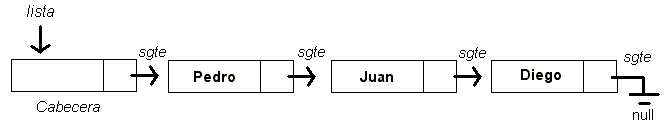
\includegraphics[width=0.5\textwidth]{lista}
\\\cite{4}
\\\textit{Representación de un TDA tipo lista enlazada}.
\end{center}
%[4] https://users.dcc.uchile.cl/~bebustos/apuntes/cc30a/TDA/listaEnlazada.gif

%%%%%%%%%%%%%%%%%%%%%%%%%%%%%
La aplicación fue realizada en Android Studio el cual es el entorno de desarrollo integrado oficial para la plataforma Android. Fue anunciado el 16 de mayo de 2013 en la conferencia Google I/O, y reemplazó a Eclipse como el IDE oficial para el desarrollo de aplicaciones para Android. La primera versión estable fue publicada en diciembre de 2014.\cite{5}

Android Studio está basado en el software IntelliJ IDEA de JetBrains y ha sido publicado de forma gratuita a través de la Licencia Apache 2.0. Está disponible para las plataformas Microsoft Windows, macOS y GNU/Linux. Ha sido diseñado específicamente para el desarrollo de Android.\cite{5}

%[5] https://developer.android.com/studio/releases/

%En este texto se muestra como se debe citar a una página de internet: %\cite{anatohipervisor}. LA pagina debe llevar por lo menos 3 campos: Autor o %título (en algunos casos el autor no es visible, solo incluir título, URL y %fecha de consulta (en automático se incluye la fecha del documento). 

%Tambien es posible citar artículos científicos, reportes técnicos y tesis de %licenciatura o maestría. En algunos casos también es posible incluir libros, %pero todos estos ITEMS no deben llevar enlace, sino que se deben investigar los %datos de la publicación (ver ejemplos de citas en este documento). 
\section{Desarrollo Experimental}
En este trabajo se desarrolló una aplicación móvil para el S.O Android en el lenguaje de programación Java, el cual permite simular un TDA o lista enlazada, pudiendo realizar operaciones de inserción tanto al principio y al final de la lista, asi como elminación al principio y final de esta tambien por parte del usuario. Ademas de esto, el usuario puede realizar una búsqueda de un elemento y la aplicación muestra en que posiciones se encuentra el elemento que se ingreso en el criterio de busqueda, es decir si se ingresa como entrada el elemento \textbf{X}, la aplicación mostrara la posición o posiciones en las que se encuentra este elemento en la lista empezando obviamente desde la posición \textbf{0}. \\
Para la realización de la aplicación, se investigó acerca de sintaxis del lenguaje de programación Java, ademas de la instalación del JDK de Java y SDK de Android Studio. Ademas de esto, se tuvo que investigar acerca de los TDA y listas enlazadas para poder conocer como estan estructuradas, como funcionan y familiarizarse con las operaciones que se les pueden realizar a estas. Una vez investigados estos temas, se procedió a realizar un análisis detallado acerca de los requerimientos de la práctica y la entrada que recibirá la aplicación. En este caso en particular, la entrada por parte del usuario es un \textit{elemento} de cualquier tipo de dato. Posteriormente, se colocaron botones en el Layout de la aplicación los cuales permiten; \textit{Insertar al frente de la lista} (inserta el elemento al principio), \textit{insertar al final de la lista} (inserta el elemento al final), \textit{eliminar al frente de la lista} (elimina el primer elemento), \textit{eliminar al final de la lista} (elimina el ultimo elemento) y finalmente \textit{buscar}, ademas de dos controles de tipo \textit{TextView}, en uno se visualiza el estado de la lista actual y en el otro se visualiza el resultado de la búsqueda. Finalmente se tiene un control de tipo \textit{EditText} el cual corresponde a la entrada de la aplicación, es decir el usuario ingresa la entrada en esa caja de texto.\\
Despues de realizar el diseño de la aplicación se procedió a colocar dos líneas de código las cuales corresponden a la petición de permisos de escritura y lectura de archivos en Android. Esto debido a que es necesario guardar la lista enlazada en un archivo con extensión \textbf{txt}. Las líneas son las siguientes:\\

\textit{ \url{<uses-permission android:name="android.permission.WRITE_EXTERNAL_STORAGE"></uses-permission>
    <uses-permission android:name="android.permission.READ_EXTERNAL_STORAGE"></uses-permission>}}\\

Ademas de esto, se utilizaron algunas funciones para la peticion de permisos al usuario para lectura y escritura de archivos. Lo anterior dicho fue obtenido de un demo presentado en clase.\\

Cabe destacar que se utilizo el demo proporcionado en clase, en el cual se implementa la escritura y lectura de archivos de texto del almacenamiento interno del dispositivo. Por lo que se implemento parte de este código. \\
Sabiendo que la única entrada de texto por parte del usuario es un \textit{elemento} elemento de cualquier tipo, se realizó una función de validación la cual consiste básicamente en verificar que el elemento no esté vacío.\\
Como paso inicial para la lectura y escritura de datos, primeramente, se hizo uso de una función que consiste en la creación del archivo de texto en el directorio en caso de que el este no exista. En dicho archivo se guardará la lista enlazada. Posteriormente, se procedió a diseñar y programar un algoritmo que, en base un nombre de archivo, realiza la lectura de este en el directorio señalado y posteriormente, lee cada línea del archivo de texto y almacena en un \textit{ArrayList} cada linea que contiene este (cada linea corresponde a un elemento de la lista enlazada).\\

Posteriormente se procedió a programar las funciones encargadas de realizar operaciones a la lista enlazada. Primeramente se realizó la función \textit{insertar al frente}, para ello se diseñó e implementó por cuenta propia, un algoritmo, el cual dado un \textit{ArrayList} que contiene los elementos de la lista enlazada leídos desde el archivo de texto en el almacenamiento, se crea un nuevo \textit{ArrayList} del tamaño de la lista anterior + 1, posteriormente se realiza la inserción del elemento que fue dado de entrada por parte del usuario en la primera posición del nuevo \textit{ArrayList} y posteriormente se trasladan los elementos restantes de la lista original a la nueva lista mediante un ciclo for, actualizando las posiciones a \textit{i + 1}, en donde \textit{i} es la posición original del elemento de la lista antigua. Posteriormente se remplaza el contenido del archivo de texto que almacena la lista con la nueva lista creada de tal manera que cada elemento se coloca en una línea del archivo de texto y se procede a guardar el contenido del este.\\

La siguiente función que se realizó fue la de \textit{insertar al final}, la cual consiste en insertar un elemento al final de la lista enlazada. Para realizar esto se diseño e implementó un algoritmo muy similar al anterior. De igual manera, se lee el archivo de texto del almacenamiento el cual contiene la lista enlazada despues de realizar alguna operación y se obtiene un \textit{ArrayList} el cual contiene los elementos de la lista y posteriormente, se crea un nuevo \textit{ArrayList} el cual corresponde a la nueva lista del tamaño de la lista anterior + 1. Despues de esto, se trasladan todos los elementos de la lista antigua a la lista nueva mediante un ciclo for, y finalmente, en la ultima posición de esta se inserta el elemento dado de entrada por el usuario. Posteriormente se procede a guardar la lista en el archivo de texto.\\

Despues de esto se realizó la función \textit{eliminar al frente}, la cual consiste en borrar el primer elemento de la lista enlazada. Para realizar esto se diseño e implementó un algoritmo, de igual manera, se lee el archivo de texto del almacenamiento el cual contiene la lista enlazada despues de realizar alguna operación y se obtiene un \textit{ArrayList} el cual contiene los elementos de la lista y posteriormente, se crea un nuevo \textit{ArrayList} el cual corresponde a la nueva lista del tamaño de la lista anterior - 1. Despues de esto, se trasladan todos los elementos de la lista antigua a partir de la \textbf{posición 1} a la lista nueva mediante un ciclo for con inicio en \textit{i = 1 hasta i menor o igual al tamaño del ArrayList antiguo}, de tal manera que se excluye el elemento en la posición 0. Posteriormente se procede a guardar la lista en el archivo de texto.

La siguiente función que se realizó fue \textit{eliminar al final}, la cual consiste en borrar el ultimo elemento de la lista enlazada. Para realizar esto se diseño e implementó un algoritmo, de igual manera, se lee el archivo de texto del almacenamiento el cual contiene la lista enlazada despues de realizar alguna operación y se obtiene un \textit{ArrayList} el cual contiene los elementos de la lista y posteriormente, se crea un nuevo \textit{ArrayList} el cual corresponde a la nueva lista del tamaño de la lista anterior - 1. Despues de esto, se trasladan todos los elementos de la lista antigua a partir de la \textbf{posición 0} a la lista nueva mediante un ciclo for con inicio en \textit{i = 0 hasta i menor al tamaño del ArrayList antiguo disminuido en una unidad}, de tal manera que se excluye el elemento en la ultima posición del \textit{ArrayList} antiguo. Posteriormente se procede a guardar la lista en el archivo de texto.

%Falta funcion buscar


Otra de las funciones que se realizaron fue la de \textit{buscar elemento}, la cual consiste en dado un elemento de entrada, se procede a verificar los elementos de la lista, si alguno(os) coinciden con este, se guarda la/las posicion(es) en donde se encuentra. Para realizar esto se diseño e implementó un algoritmo, de igual manera, se lee el archivo de texto del almacenamiento el cual contiene la lista enlazada despues de realizar alguna operación y se obtiene un \textit{ArrayList} el cual contiene los elementos de la lista y posteriormente, se realiza un ciclo for, el cual accedera a cada uno de los elementos del ArrayList y verifica si es igual al elemento dado de entrada, de ser cierto, se guarda la posicion y asi con todos los elementos. Finalmente esta funcion muestra al usuario a traves del \textit{EditText} de busqueda que posiciones o posicion hicieron match con el elemento ingresado.

Es importante mencionar que, se realizaron funciones auxiliares como lo es \textit{showList} la cual lee el archivo de texto del directorio y muestra en pantalla la lista enlazada. Esta funcion es ejecutada cada vez que se realiza alguna operación a la lista, para que la visualizacion de esta sea actualizada.

De igual manera, al realizar alguna operación a la lista o alguna busqueda, se es guardado en otro archivo de texto en el directorio, el registro de las operaciones realizadas a la lista. Para ello, se tuvo que diseñar e implementar un algoritmo que, dada una operación realice una escritura en un archivo de texto dado un nombre, en este caso el nombre del archivo es log Por lo que cualquier usuario con una aplicación de administración de archivos puede localizar este y el archivo en el que se almacena la lista en el directorio siguiente: \texttt{\detokenize{Almacenamiento Interno / Problema8_CDM}}, dentro de esta carpeta se encuentra el archivo \texttt{\detokenize{lista_enlazada.txt}} y \texttt{\detokenize{log.txt}}.

Para ver un panorama más general del proceso realizado, a continuación se muestra un diagrama de flujo:
\begin{center}
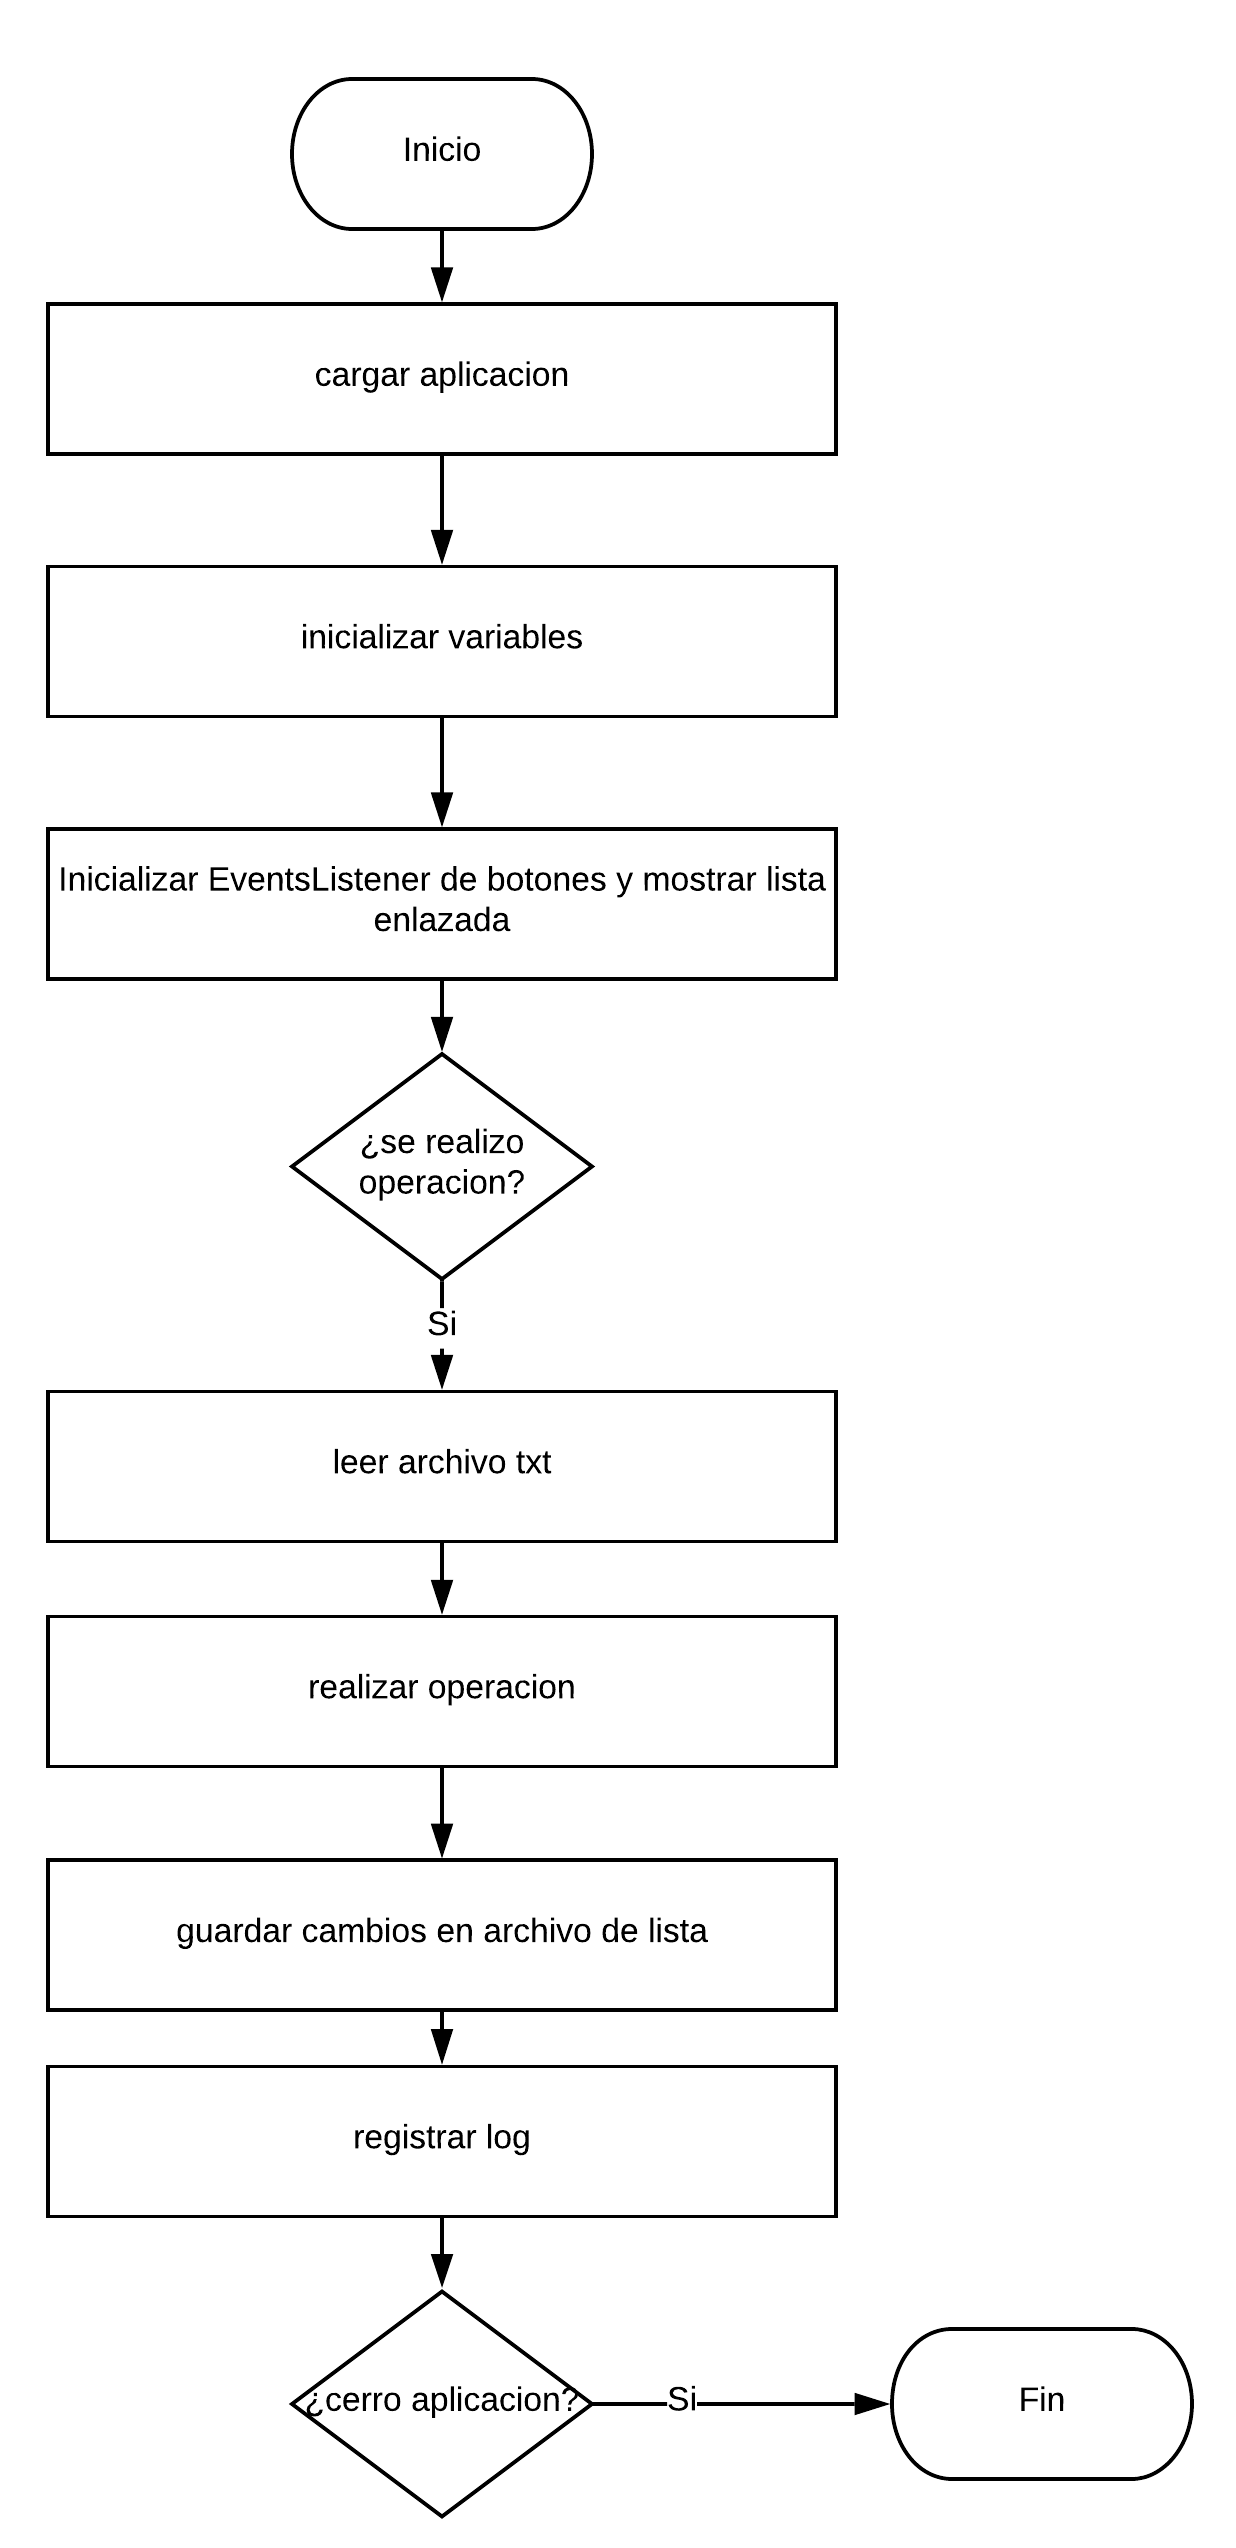
\includegraphics[width=0.5\textwidth]{flujo}
\\\textit{Diagrama de flujo de la aplicacion}.
\end{center}
\section{Resultados}
El programa deberá compilarse de la siguiente manera:



Después de ejecutarlo aparecerá en consola lo siguiente, lo cual es información e instrucciones del uso del programa:



Abrimos la ventana de nuestro programa y nos encontraremos con lo siguiente:

En donde aparece la información del desarrollador y los controles, con la tecla + se podrá cambiar las medidas de los lados del cuadrado y con la tecla escape (ESC) se cierra el programa. Así como también, la pantalla nos muestra las longitudes de lado de cada cuadrado(a longitud del cuadrado A y así sucesivamente). Además, nos encontramos con los dos lados de los cuadrados que podemos mover. Los puntos en color negro corresponden a vértices de los cuadrados, usted puede dar clic y moverlos a razón de radio de una circunferencia. A continuación se procede a intentar a unir (debido a que no en todos los casos será posible) para formar el triángulo y obtener el ángulo entre las dos semirrectas.


Una vez unidos los vértices (lados juntos) se colorea el triángulo formado con color azul y se muestra la medida del ángulo que en este caso fue de 60.94 grados.

Si queremos cambiar las medidas o reiniciar el simulador se presiona la tecla +. Finalmente presionamos la tecla escape para salir.


\section{Conclusión}

En este trabajo se ha dado solución a un simulador de tres cuadrados mediante el cual, dada la medida de sus lados, se puede saber si pueden o no formar un triángulo con estos y calcular el ángulo comprendido entre dos de sus rectas. Para lograr esto se tuvo que realizar una investigación acerca de diversos temas relacionados con la trigonometría y fórmulas para calcular puntos o pendientes de rectas, así como también sobre el lenguaje C++. En el desarrollo de este programa se pusieron en práctica habilidades de investigación y análisis.


\section*{Referencias}
[1] Triángulo,\url{http://www.universoformulas.com/matematicas/geometria/triangulo/}, visitado 08/10/2017

[2] Concepto de triángulo,\url{http://conceptodefinicion.de/triangulo/}, visitado 08/10/2017

[3] Ángulos,\url{https://www.smartick.es/blog/matematicas/recursos-didacticos/angulos-i/}, visitado 08/10/2017

[4] Funciones trigonométricas,\url{ https://sites.google.com/site/magiamatematica2015/funciones-trigonometricas}, visitado 08/10/2017

[5] Imagen función trigonométrica,\url{https://es.wikipedia.org/wiki/Funcion_trigonometrica}, visitado 08/10/2017


\end{document}














